%%%% Paramétrage du cours %%%%
\def\xxactivite{Cours}
\def\xxauteur{\textsl{Xavier Pessoles}}

\fichefalse
\proftrue
\tdfalse
\courstrue

\def\xxnumchapitre{Chapitre 2 \vspace{.2cm}}
\def\xxchapitre{\hspace{.12cm} Systèmes séquentiels}


\def\xxcompetences{%
\textsl{%
\textbf{Savoirs et compétences :}\\
\begin{itemize}[label=\ding{112},font=\color{ocre}] 
\item ** %B2-10 : Déterminer les caractéristiques d'un solide ou d'un ensemble de solides indéformables.
\end{itemize}
}}


\def\xxfigures{
\begin{center}
\includegraphics[width=.95\textwidth]{fig_0a}

\vspace{1cm}

\includegraphics[width=.95\textwidth]{fig_0b}

\vspace{1cm}

\includegraphics[width=.95\textwidth]{fig_0c}
%\textit{Digicode}
\end{center}
}%figues de la page de garde

\input{\repStyle/new_pagegarde}

\setlength{\columnseprule}{.1pt}

\vspace{2cm}
\pagestyle{fancy}
\thispagestyle{plain}

%%%%%%%%%%%



%%%%%%%%%%%%%%%%%%%%%%%%%%%%%%%%%%%%%
\section{La fonction mémoire}

\subsection{Le chronogramme}
Le chronogramme est un outil permettant d'afficher l'état des entrées et des sorties en fonction du temps. Le chronogramme suivant indique le fonctionnement d'une lampe. L'interrupteur <<va-et-vient>> est relié à un relais. 

\begin{minipage}[c]{.47\linewidth}
\begin{center}
\includegraphics[width=.9\textwidth]{Chrono1}
\end{center}
\end{minipage} \hfill
\begin{minipage}[c]{.47\linewidth}
\begin{center}
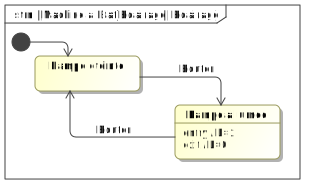
\includegraphics[width=.95\textwidth]{Eclairage}
\end{center}
\end{minipage}

Ainsi, pour une même combinaison des entrées, on observe des états différents de la sortie.

Le même constat peut être dresser à partir du fonctionnement d'un moteur (\textit{Exemple : fonctionnement du système Doshydro}).


\begin{minipage}[c]{.47\linewidth}
\begin{center}
\includegraphics[width=.9\textwidth]{Chrono2}
\end{center}
\end{minipage} \hfill
\begin{minipage}[c]{.47\linewidth}
\begin{center}
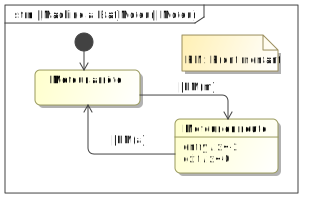
\includegraphics[width=.95\textwidth]{Moteur}

\includegraphics[width=.95\textwidth]{Moteur_im}
\end{center}
\end{minipage}

Ici aussi, on remarque qu'une même combinaison des entrées ($a=m=0$) peut conduire à un état de marche ou d'arrêt du moteur. Une variable interne, ici, une mémoire, permet de mémoriser l'état du moteur. 

\subsection{Notion de mémoire}

La mémorisation des états est à la base de l'existence des systèmes séquentiels. En notant $x$ la variable interne d'un système, on lui associe une mémoire.

 On peut noter l'existence des mémoires permanentes (qui conservent l'état des variables en cas de coupure d'énergie) et les mémoires volatiles (qui perdent l'état des variables en cas de coupure d'énergie).  
 
 Les mémoires peuvent être réalisées de façon optique (blue-ray), électropneumatiques (distributeurs électropneumatiques bistables), mangnétiques (disques durs), électriques (grâce à des transistors, mémoire flash), électromagnétique (relais). 
 
 Dans les systèmes automatisés industriels, le relais auto maintenu électromagnétique est un élément clef de la mémorisation des états. 

\begin{center}
\includegraphics[width=\textwidth]{relais}
\end{center}

Lorsque l'utilisateur presse le bouton $m$, le relais $X$ est activé. Ainsi, la variable $x$ est mise à 1 ce qui provoque l'éclairage de la lampe $L$. \'A ce stade, si on relâche l'interrupteur $m$ le relais $X$ est désactivé, la variable $x$ passe à l'état 0 et la lampe s'éteint.

\begin{obj}
Comment réaliser une mémoire par l'utilisation d'un relais ? 
Que se passe-t-il lors de l'appui simultané sur marche et arrêt. 
\end{obj}

\subsection{Réalisation d'une mémoire}
\subsubsection*{Exmple : mémoire à effacement prioritaire}
Dans ce cas, le moteur s'allume lorsque $m$ est pressé. Il est éteint lorsque $a$ est pressé ou lorsque $m$ et $a$ sont pressés simultanément.
 
 
\begin{minipage}[c]{.5\linewidth}
\begin{center}
\includegraphics[width=\textwidth]{mem_eff}
\end{center}
\end{minipage} \hfill
\begin{minipage}[c]{.47\linewidth}
Il est possible de traduire le fonctionnement du moteur par l'équation booléenne suivante : 
$$
M = \overline{a} \cdot \left(m +  x \right)
$$
Ainsi dans un premier temps, en appuyant sur $m$ le relais est actionné, $x$ passe donc à 1 dans le circuit de puissance (allumant ainsi le moteur) \textbf{et} dans le circuit de commande. On effectue ainsi un \textbf{auto maintien}. 

On comprend aisément qu'un appui simultané sur $a$ et $m$ provoque une désactivation du relais et donc un arrêt du moteur. 
\end{minipage}

\vspace{.2cm}

Lorsqu'on utilise une technologie électronique, il est courant d'utiliser de réaliser un câblage en utilisant des cellules NOR. 

\vspace{.2cm}

\begin{minipage}[c]{.3\linewidth}
\begin{center}
\includegraphics[width=\textwidth]{mem_eff_nor}
\end{center}
\end{minipage} \hfill
\begin{minipage}[c]{.2\linewidth}
\begin{center}
\begin{tabular}{|c|c|c||c|}
\hline
m & a & x & Q \\
\hline \hline
0 & 0 & 0 & 0 \\\hline
0 & 0 & 1 & 1 \\\hline
0 & 1 & 0 & 0 \\\hline
0 & 1 & 1 & 0 \\\hline
1 & 0 & 0 & 1 \\\hline
1 & 0 & 1 & 1 \\\hline
1 & 1 & 0 & 0 \\\hline
1 & 1 & 1 & 0 \\\hline
\end{tabular}
\end{center}
\end{minipage} \hfill
\begin{minipage}[c]{.4\linewidth}
Il  n'est pas directement possible d'écrire directement la table de vérité de la sortie $Q$ en fonction de $a$ et de $b$. Il faut avoir recours à une variable interne $x$. 

On retrouve bien l'équation précédente : 
$$
Q = \overline{m}\cdot \overline{a} \cdot x + \underbrace{m\cdot \overline{a} \cdot \overline{x} 
+ m\cdot \overline{a} \cdot x}_{m\cdot \overline{a} } 
$$

$$Q
= \overline{a} \left(\overline{m} \cdot x + m\right)
= \overline{a} \left( x + m\right)
$$

\end{minipage}
%
%\paragraph*{Les bascules}
%Le montage précédent est appelé une bascule SR (Set -- Reset). Suivant les cas d'utilisation, il en existe plusieurs. 
%   
%  
%\vspace{.2cm}
%
%\begin{minipage}[c]{.15\linewidth}
%\begin{center}
%\includegraphics[width=\textwidth]{basculeRS}
%\end{center}
%\end{minipage} \hfill
%\begin{minipage}[c]{.2\linewidth}
%\begin{center}
%\begin{tabular}{|c|c||c|c|}
%\hline
%$S$ & $R$ &  $Q_n$ & $\overline{Q_{n}}$ \\
%\hline \hline
%0 & 0 & $Q_{n-1}$ & $\overline{Q_{n-1}}$ \\ \hline
%0 & 1 & 0 & 1 \\\hline
%1 & 0 & 1 & 0 \\\hline
%1 & 1 & 0 & 0 \\\hline
%1 & 1 & -- & -- \\\hline
%\end{tabular}
%\end{center}
%\end{minipage} \hfill
%\begin{minipage}[c]{.53\linewidth}
%La bascule RS est caractérisée par deux états : 
%\begin{itemize}
%\item S (Set) caractérise <<la mise à 1>>;
%\item R (Reset) caractérise <<la mise à 0>>.
%\end{itemize}
%
%$Q_n$ et $\overline{Q_n}$ caractérisent les deux sorties stables. La combinaison $S=R=1$ est à éviter car elle conduit à des dysfonctionnement. Pour palier à ce problème, on utilise une bascule JK. 
%\end{minipage}
%   	
%  \vspace{.2cm}
%\hfill
%\begin{minipage}[c]{.15\linewidth}
%\begin{center}
%\includegraphics[width=\textwidth]{basculeJK}
%\end{center}
%\end{minipage} \hfill
%\begin{minipage}[c]{.4\linewidth}
%\begin{center}
%\includegraphics[width=\textwidth]{basculeJK_logi}
%\end{center}
%
%\end{minipage} \hfill
%\begin{minipage}[c]{.35\linewidth}
%
%\begin{center}
%\begin{tabular}{|c|c||c|c|}
%\hline
%$J$ & $K$ &  $Q_n$ & $\overline{Q_{n}}$ \\
%\hline \hline
%0 & 0 & $Q_{n-1}$ & $\overline{Q_{n-1}}$ \\ \hline
%0 & 1 & 0 & 1 \\\hline
%1 & 0 & 1 & 0 \\\hline
%1 & 1 & 0 & 0 \\\hline
%1 & 1 & $Q_{n-1}$ & $\overline{Q_{n-1}}$ \\\hline
%\end{tabular}
%\end{center}
%\end{minipage}\hfill

\section{Modélisation du comportement des systèmes séquentiels -- Diagrammes d'états \cite{1}}

L'outil SysML privilégié pour décrire le fonctionnement d'un système séquentiel sera le diagramme d'état.

Le diagramme de séquence permet de présenter la succession d'étapes liés à un cas d'utilisation d'un point de vue utilisateur. Le diagramme d'état et le diagramme d'activité permettent de décrire l'évolution interne du système. 
                           

\subsection{États -- transition}
\begin{defi}
Un état caractérise la situation d'un système à un moment donné. Pour passer d'un état à l'autre,  utilise des transitions. La succession étape -- transition donne donc un diagramme d'états. 

\begin{center}
\includegraphics[width=.8\textwidth]{stm_def}
\end{center}

Dans un premier temps on peut définir 3 pseudo-états : 
\begin{itemize}
\item le pseudo-état initial, unique et indispensable, marque le point de départ du diagramme d'état;
\item les pseudo-états intermédiaires décrivent le comportement du système pour un cas d'utilisation attendu;
\item le pseudo-état final (non obligatoire) marque la fin d'un cas d'utilisation.
\end{itemize}

\textbf{Dans un diagramme d'état, UN SEUL ÉTAT est actif à la fois.}

Pour passer d'un état à l'autre, on utilise des transitions. À ces transitions on peut associer les éléments (facultatifs) suivants :
\begin{itemize}
\item un événement : celui-ci est l'élément déclencheur pour utiliser la transition. S'il est absent, il faudra attendre la fin de l'état pour utiliser la transition;
\item une condition de garde (entre crochet) : il s'agit d'une conditions booléennes à évaluer lorsque l'événement est déclenché. Si l'événement est déclenché \textbf{et si} la condition de garde est vraie \textbf{alors} la transition est franchie;
\item l'effet : il s'agit d'une action exécutée au passage de la transition. 
\end{itemize}
\end{defi}
%\begin{methode}
%  Pour chaque diagramme, il faut définir un état représenté par un n\oe{}ud. Au cas où
%aucune activité n’est souhaitée, c’est un état d’attente.
%
%Il faut ensuite identifier les cas d’évolution du système, c'est-à-dire les transitions
%possibles d’un état à un autre. On trace alors un lien entre les n\oe{}uds
%correspondants. Chaque transition peut être qualifiée par un évènement, une
%condition de garde et un effet.
%\end{methode}
%
\begin{exemple}
\textit{Commande tout ou rien d'un moteur}

\vspace{.2cm}
\noindent
\begin{minipage}[c]{.48\linewidth}
Deux états internes du système cohabitent. Dans un cas le moteur est en marche, dans l’autre il est à l’arrêt.

Les conditions de passage d’un état à un autre se font à l’aide des variables d’entrée arrêt « a » et marche « m ».


L’activité « Marche moteur » peut être détaillée dans un diagramme d’activité. Elle comporterait l’action « distribuer l’énergie ». Son exécution ne nécessite pas de temps significatif, elle est associée à un ordre de commande en direction du préactionneur du moteur (un contacteur électrique à arrêt prioritaire).
\end{minipage} \hfill
\begin{minipage}[c]{.46\linewidth}
\begin{center}
\includegraphics[width=\textwidth]{Commandemoteur}
\end{center}
\end{minipage}

\end{exemple}


\begin{defi}[Activité, action]

En SysML une activité a la propriété de durer un certain temps. Une action est quant à elle instantanée. 

\end{defi}
\subsection{Utilisation des pseudo-états}


\begin{defi}
Les pseudo-états permettent d’utiliser des fonctionnalités avancées sans trop compliquer le diagramme d’état avec le formalisme de base.
Il est alors possible de montrer des sélections de séquences d’états (évolutions avec alternatives), des structures parallèles (évolutions simultanées), \textit{etc}.
\end{defi}

\begin{exemple}

\textit{Commande tout ou rien (TOR) d’un moteur}

Un diagramme d’états «~choix de mode~» de niveau hiérarchique supérieur à celui décrit précédemment («~commande moteur~»), permet de le démarrer selon deux modes :
\begin{itemize}
\item « mode normal » : moteur à l’arrêt dans l’« état d’attente »;
\item « mode historique » : dernier état avant que l’on sorte du diagramme « commande moteur » (« état d’attente » ou « état de marche »).
\end{itemize}

\begin{center}
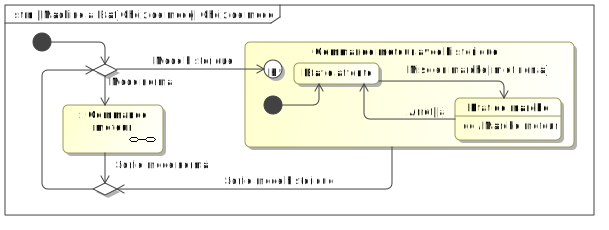
\includegraphics[width=.8\textwidth]{ChoixMode}
\end{center}
\end{exemple}

\subsection{États composites}
On ne rentrera pas dans le détail des états composites. Ceux-ci permettent de regrouper, à l'intérieur même d'un état, plusieurs états. Ainsi, on peut retrouver dans un état composite un diagramme d'état complet.

Il existe aussi des états composites << orthogonaux >> permettant de traduire la mise en parallèles d'états. 

\section{Structures algorithmiques}
\subsection{Affectation}
L’affectation d’une valeur à une variable peut se faire à l’aide d’une action. Cela ne prend pas
de temps significatif.

\begin{minipage}[c]{.48\linewidth}
\begin{center}
\includegraphics[width=\textwidth]{etat_affectation}

\textit{Diagramme d'états -- Affectation}
\end{center}
\end{minipage} \hfill
\begin{minipage}[c]{.48\linewidth}
\begin{center}
\includegraphics[width=.75\textwidth]{activite_affectation}

\textit{Diagramme d'activité -- Affectation}
\end{center}
\end{minipage}

\subsection{Groupe d'instructions}

Un groupe ou un bloc d’instructions peut être une séquence d’un diagramme
d’activité. Cela correspond à une succession d’actions et / ou d’activités.

\begin{center}
\includegraphics[width=.5\textwidth]{GroupeInstruction}

\textit{Groupe d'instructions}
\end{center}



\subsection{Fonctions et procédures}
La décomposition d’un algorithme en fonctions et procédures, permet :
\begin{itemize}
\item d’une part, de scinder une problématique générale en plusieurs problématiques
élémentaires;
\item d’autre part, de pouvoir réutiliser des sous-programmes réalisant des tâches élémentaires.
\end{itemize}

%
%\begin{minipage}[c]{.48\linewidth}
%\begin{center}
%\includegraphics[width=\textwidth]{Fonctions_stm}
%
%\textit{Diagramme d'états -- Affectation}
%\end{center}
%\end{minipage} \hfill
%\begin{minipage}[c]{.48\linewidth}
%\begin{center}
%\includegraphics[width=.7\textwidth]{Affectation_act}
%
%\textit{Diagramme d'activité -- Affectation}
%\end{center}
%\end{minipage}

Une procédure comporte une succession d’instructions mais ne renvoie rien.
\'A la fin de l’exécution d’une fonction, il y a le retour d’une valeur, d’une liste, d’un objet, etc.
\subsection{Structure alternative (conditionnelle)}

\begin{minipage}[c]{.48\linewidth}
\begin{center}
\includegraphics[height=4cm]{Condition_stm}

\textit{Diagramme d'états -- Structure alternative complète}
\end{center}
\end{minipage} \hfill
\begin{minipage}[c]{.48\linewidth}
\begin{center}
\includegraphics[height=4cm]{Condition_act}

\textit{Diagramme d'activité -- Structure alternative avec saut}
\end{center}
\end{minipage}

\subsection{Structure répétitive (itérative)}
\begin{minipage}[c]{.48\linewidth}
\begin{center}
\includegraphics[height=4cm]{Iteratif_stm}

\textit{Diagramme d'états -- Tant que condition vraie faire ...}
\end{center}
\end{minipage} \hfill
\begin{minipage}[c]{.48\linewidth}
\begin{center}
\includegraphics[height=4cm]{Iteratif_act}

\textit{Diagramme d'activité -- Répéter... jusqu'à condition vraie}
\end{center}
\end{minipage}


\begin{exemple}
Pour variable = valeur initiale, jusqu'à valeur maximale, faire...
\end{exemple}

\begin{minipage}[c]{.48\linewidth}
\begin{center}
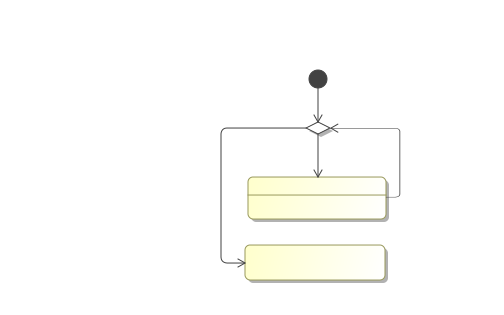
\includegraphics[height=5cm]{Compteur}

\textit{Diagramme d'états}
\end{center}
\end{minipage} \hfill
\begin{minipage}[c]{.48\linewidth}
\begin{center}
\includegraphics[height=5cm]{compteur_act}

\textit{Diagramme d'activité}
\end{center}
\end{minipage}

\begin{thebibliography}{2}
\bibitem{sg}{Stéphane Genouël, \textit{Systèmes Séquentiels -- Fonction mémoire}, Cours de MPSI -- PCSI, Lycée Chateaubriand, Rennes, \url{http://stephane.genouel.free.fr/}.} 
\bibitem{pb}{Patrick Beynet et Al., \textit{Sciences Industrielles pour l'Ingénieur, MPSI -- PCSI}, Éditions Ellipses.}
\bibitem{3}{Pierre Debout, \textit{Automatique -- Systèmes à événements discrets}, Cours de PCSI.}
\bibitem{4}{Thierry Schanen, \textit{Guide des automatismes 9.1}, Pos Industry, 2009.}
\bibitem{5}{Olivier Le Gallo, Systèmes à événements discrets, Lycée Clémenceau, Nantes, \url{http://olivier.legallo.pagesperso-orange.fr/documents/SED.pdf}.}
\end{thebibliography}

\end{document}




